\documentclass[12pt, letterpaper]{article}
\usepackage[english]{babel}
\usepackage{graphicx}
\usepackage{float}
\usepackage{hyperref}

\title{DAT510 - Assignment 2}
\author{Fr\o ydis J\o rgensen}

\begin{document}
\begin{titlepage}
\maketitle
\end{titlepage}

\begin{abstract}
A one-paragraph summary of the entire assignment - your choices of cryptographic primitives and their parameters,
procedure, test results, and analysis. 
\end{abstract}

\section*{Introduction}
A description of the scientific background for your project, including previous work that your project builds on.
(Remember to cite your sources!) The final sentence (analogous to the thesis statement in a term paper) is the
objective of your experiment. 

\section*{Design and Implementation}
I have created both a digital signature scenario in the main with a predefined message where we can validate the signature on the message and two applications where Alice and Bob can send messages to each other with a signature and validate that the messages are correct. Both the main and the applications use the same methods and I will therefore first explain all the methods before I go into the applications. \\

When implementing RSA, I think the most crucial thing is to find some good keys. We need two random large primes, \textbf{p} and \textbf{q}. By multiplying \textbf{p} and \textbf{q} we get \textbf{n}. The keys are generated as shown in Figure \ref{fig:generatePrimes}. To decide \textbf{p} and \textbf{q} I use a package called Crypto and uses their method \textit{getPrime}, and to get a random primes I also uses Crypto's function \textit{get\_random\_bytes}. Although the chances for p and q to be the same is very small, we should make sure that's not the case. I take in the bit length as an input to the function. There are major runtime differences that depend on the bit length, but I will get back to that.

\begin{figure}[H]
  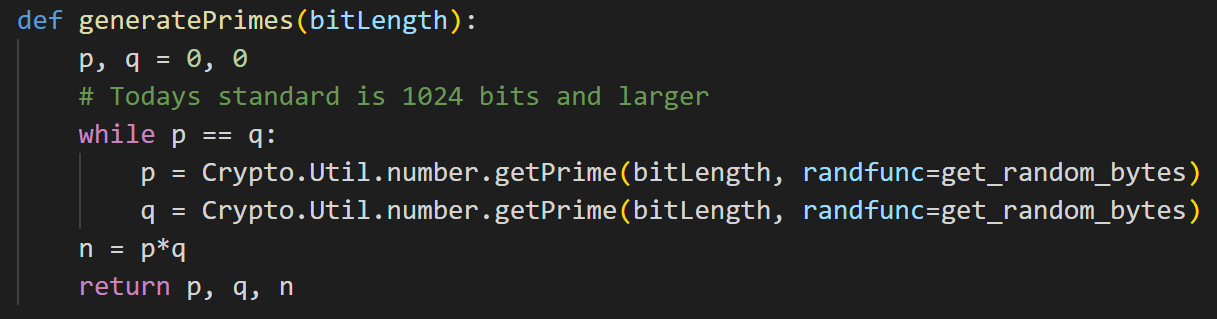
\includegraphics[width=\linewidth]{code_snippets/getPrimes.PNG}
  \caption{Generates two large primes and multiplies them}
  \label{fig:generatePrimes}
\end{figure}

The next step is to find the totient of \textbf{n}, $\phi$ phi. As shown in Figure \ref{fig:totient} that's an easy calculation using \textbf{p} and \textbf{q}.

\begin{figure}[H]
  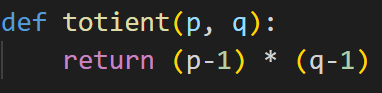
\includegraphics[width=150px]{code_snippets/totient.PNG}\centering
  \caption{Calculated the totient of n from p and q}
  \label{fig:totient}
\end{figure}

Together with \textbf{n} we have another public exponent \textbf{e}. This is a number that is the greatest common divisor of 1 with $\phi(n)$. The number in practical use is often chosen to be the Fermat number 65537. That is the largest known prime in the form of $2^{2^{n}} + 1, (n=4)$. It is large enough to avoid attacks and quick on binary calculations. But we should always check that e is not a factor of the totient $\phi$. If that is the case, we choose the next largest prime number, \cite{65537}. 
But in this assignment, we want to generate a new \textbf{e} for each time so that for testing. As shown in Figure \ref{fig:e} I use \textit{randint} to get a random number in between 3 and phi and then check that it meets the requirement. I use \textit{gcd} imported from the package math to calculate the greatest common divisor, and if the result from that is 1. We can use that number as our public key \textbf{e}. That means that \textbf{e} and $\phi$ are coprimes.

\begin{figure}[H]
  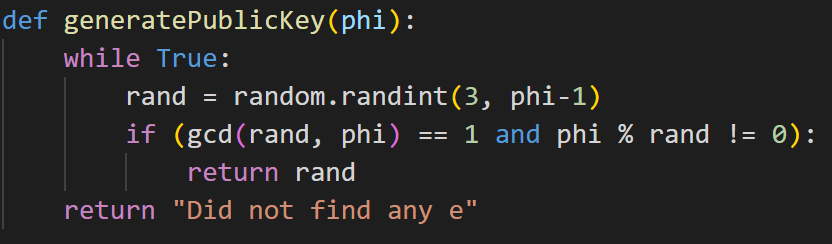
\includegraphics[width=350px]{code_snippets/gene.PNG}\centering
  \caption{generate our public component e, by finding a coprime to phi}
  \label{fig:e}
\end{figure}

Using the public exponent \textbf{e} and $\phi$ we can create the private exponent \textbf{d}. The private exponent \textbf{d} is the inverse of the public exponent with respect to the totient $\phi$. To calculate the inverse you can use the \textit{Extended Euclidean Algorithm}. I have taken an implementation of that from geeksforgeeks, ref \cite{modinv}. This method works when \textbf{e} and $\phi$ are coprimes, which we already know they are. The function to find \textbf{d} is shown in Figure \ref{fig:modinv}

\begin{figure}[H]
  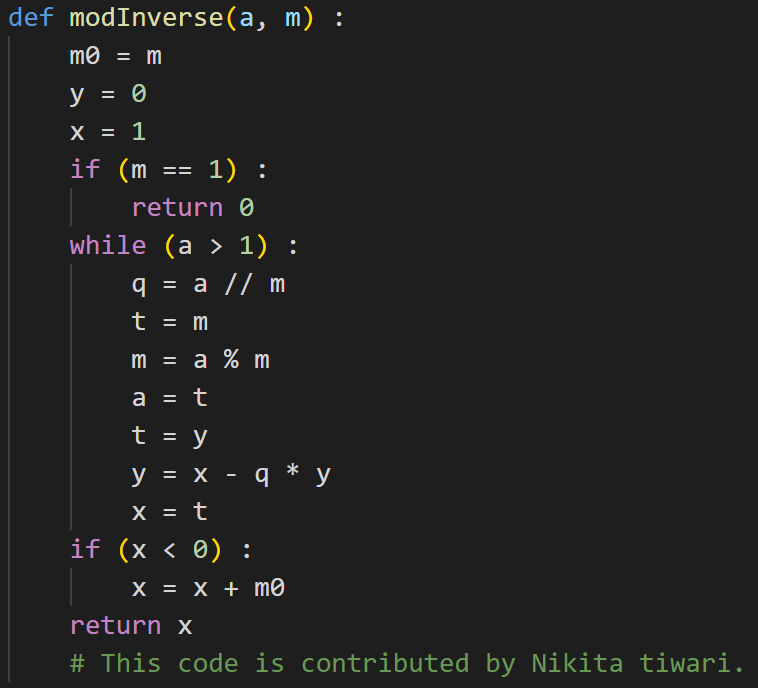
\includegraphics[width=250px]{code_snippets/modinv.PNG}\centering
  \caption{Finding the inverse. Function from GeeksforGeeks}
  \label{fig:modinv}
\end{figure}

Now that we have the public keypair of \textbf{e} and \textbf{n} and the private key pair of \textbf{d} and \textbf{n}, we can start creating the digital signature on the message. Before we can run the RSA encryption calculation to create the signature we have to hash the original data (the message). I have imported \textit{hashlib} and used SHA256 for hashing the message. So that means that no matter how long the message is, we will get a 256-bit block.
Using the hash we can now create the signature by using RSA's encryption function. We will use our private key to create the signature as shown here in the mathematical expression.
$$hash^{d}\ mod\ n$$
In the code, as shown in Figure \ref{fig:hash}, I use the function \textit{pow} which does the same as the mathematical expression. As you can also see in the figure is that I convert the hash into an integer, and throughout the program, I only work with integers instead of bits.

\begin{figure}[H]
  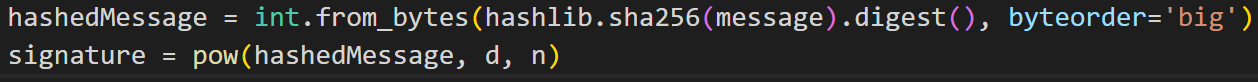
\includegraphics[width=\linewidth]{code_snippets/hash.PNG}\centering
  \caption{Hashing the message and create signature}
  \label{fig:hash}
\end{figure}

Now that we have the message and the digital signature we can send it and verify that the message is correct according to the signature and it has not been tampered by some man in the middle. To verify the signature we take the message and creates a hash using the same hashing method SHA256. This hash should match what we decrypt from the signature. To decrypt the signature we do the same mathematical operation as when it was created but instead of the message, we use the signature, and instead of the private key \textbf{d} we use the public key \textbf{e}. This works because both \textbf{e} and \textbf{n} is public keys. So in this case everyone can verify that the message was sent from f.ex Alice. Normally we would use some encryption on top of that since the message now is sent in plaintext. As you can see in Figure \ref{fig:verify}, we check that the hash we got from the message is the same that we got after decrypting the signature. If they are the same, we have verified that the message from Alice is the same as at the point Alice signed it and sent it.

\begin{figure}[H]
  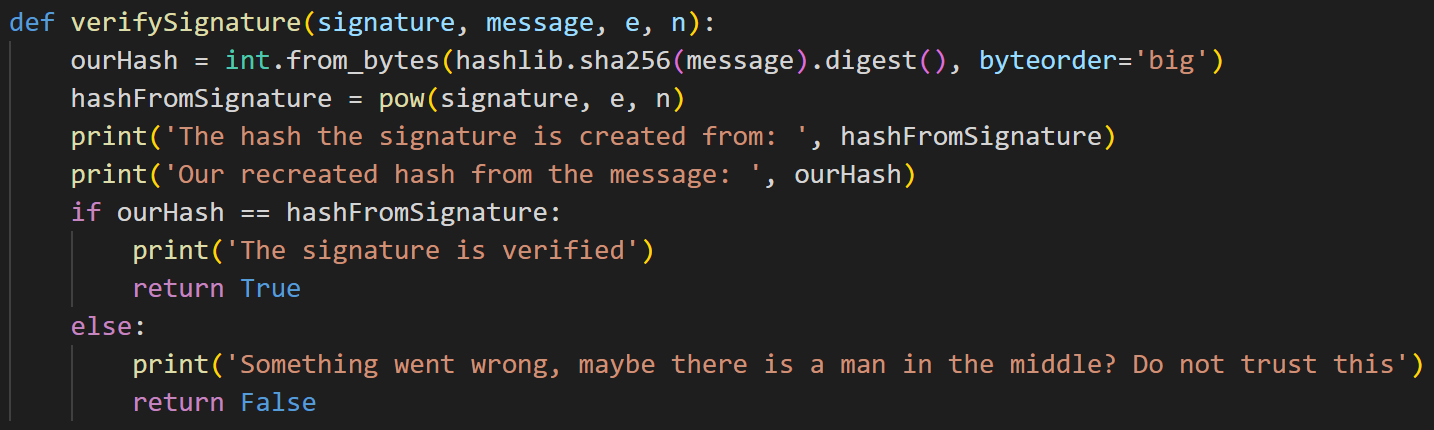
\includegraphics[width=\linewidth]{code_snippets/verify.PNG}\centering
  \caption{Verifying that the signature matches the message}
  \label{fig:verify}
\end{figure}

In the application, we have two URLs. The start URL, where we can send a message and sign it. And /getMsg where we can see the message from the other part and see if the signature is correct. \\

When a message is written and it's clicked send the keys will be created as explained previously and the signature will be created as shown in Figure \ref{fig:send}. The fetching point for people that want to receive the message is /sentMsg. And the message is sent as a dictionary including the message, the signature, \textbf{e}, and \textbf{n}.

\begin{figure}[H]
  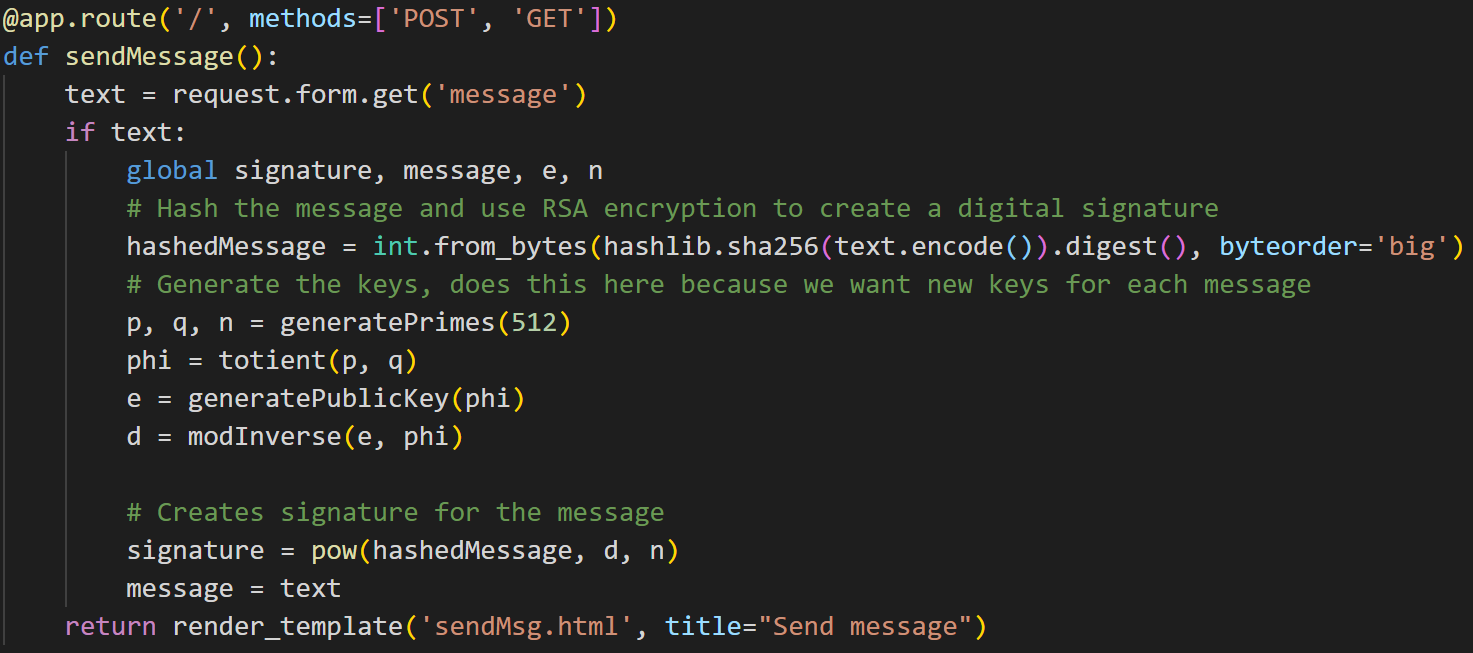
\includegraphics[width=\linewidth]{code_snippets/send.PNG}\centering
  \caption{Running a template with input field and submit button to send message with a signature}
  \label{fig:send}
\end{figure}

To fetch messages you go to /getMsg. If there is no message it will be displayed "There is no message". If there is a message we have to verify the signature. We use the \textit{verifySignature} method as shown in Figure \ref{fig:verify}. If the message and the signature correspond the message will be shown with a note that the signature is correct. If the signature is wrong there is a warning that someone might have tampered the message.
 
\begin{figure}[H]
  \hspace*{-50px}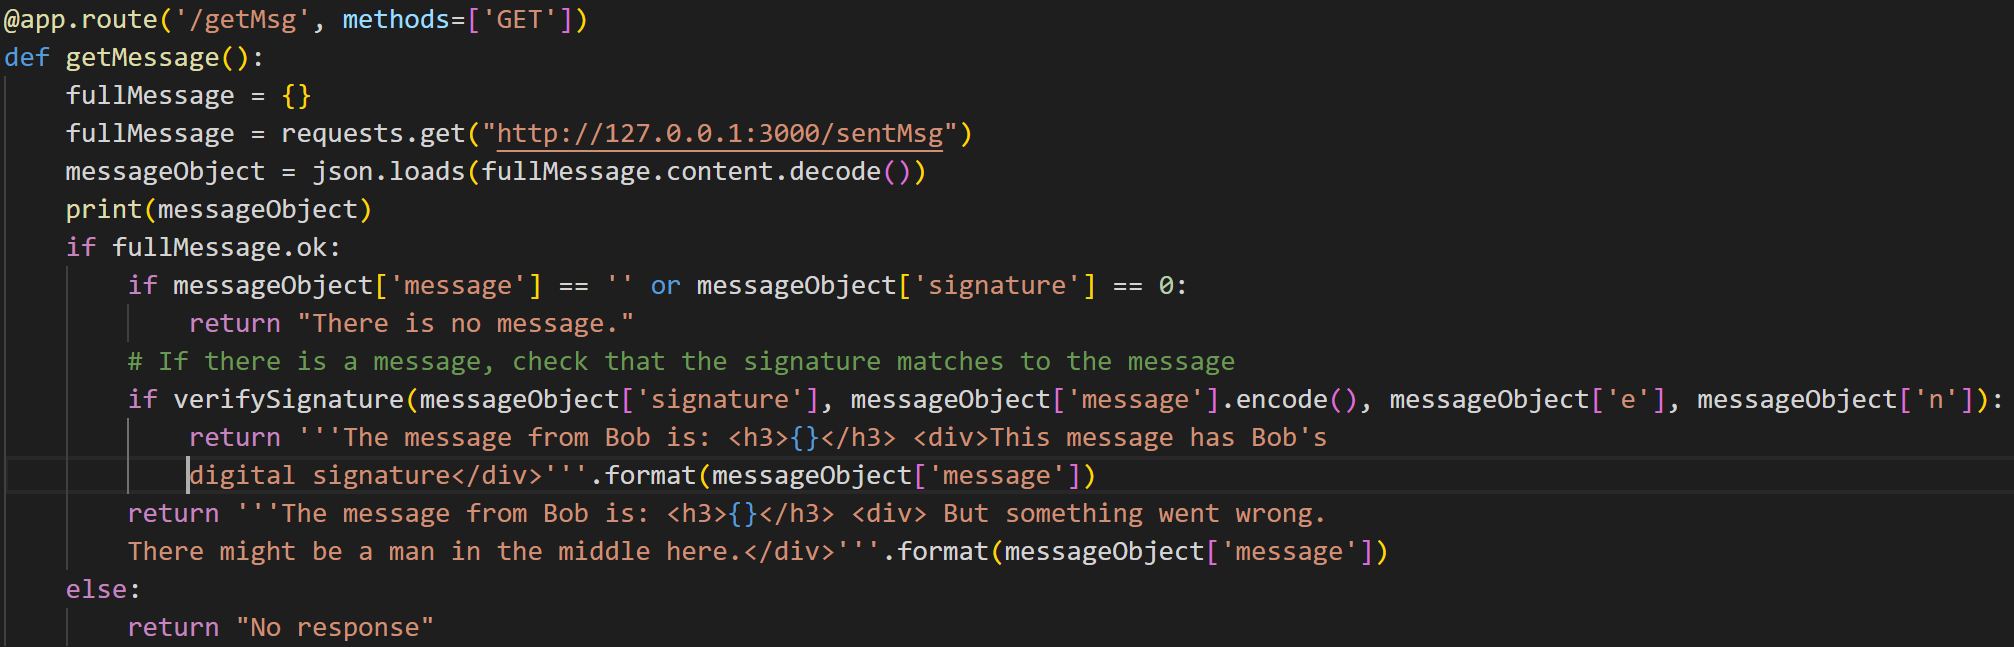
\includegraphics[width=500px]{code_snippets/get.PNG}\centering
  \caption{Fetching the message and verifying the signature}
  \label{fig:get}
\end{figure} 

The applications have a very similar set up as in assignment 2, and one is run on port 3000 and one on port 5000. 

\section*{Test results}

As in the previous assignment I created both a staged scenario and two applications to try out RSA digital signature. 
Running the main in RSA.py will print out the information we get while doing a digital signature and verifying it, in a staged scenario. As you can see in Figure \ref{fig:print}, the first thing printed is the public and private keys. Then we can see the message sent from Alice to Bob and the hashed message. From the hashed message the signature is created. The signature will be sent to Bob from Alice with the message and the public keys. Then Bob recreates a hash from the message to see that it matches the hash we got by encrypting Alice's signature. And in this case, they are the same and therefore the signature is verified.

\begin{figure}[H]
  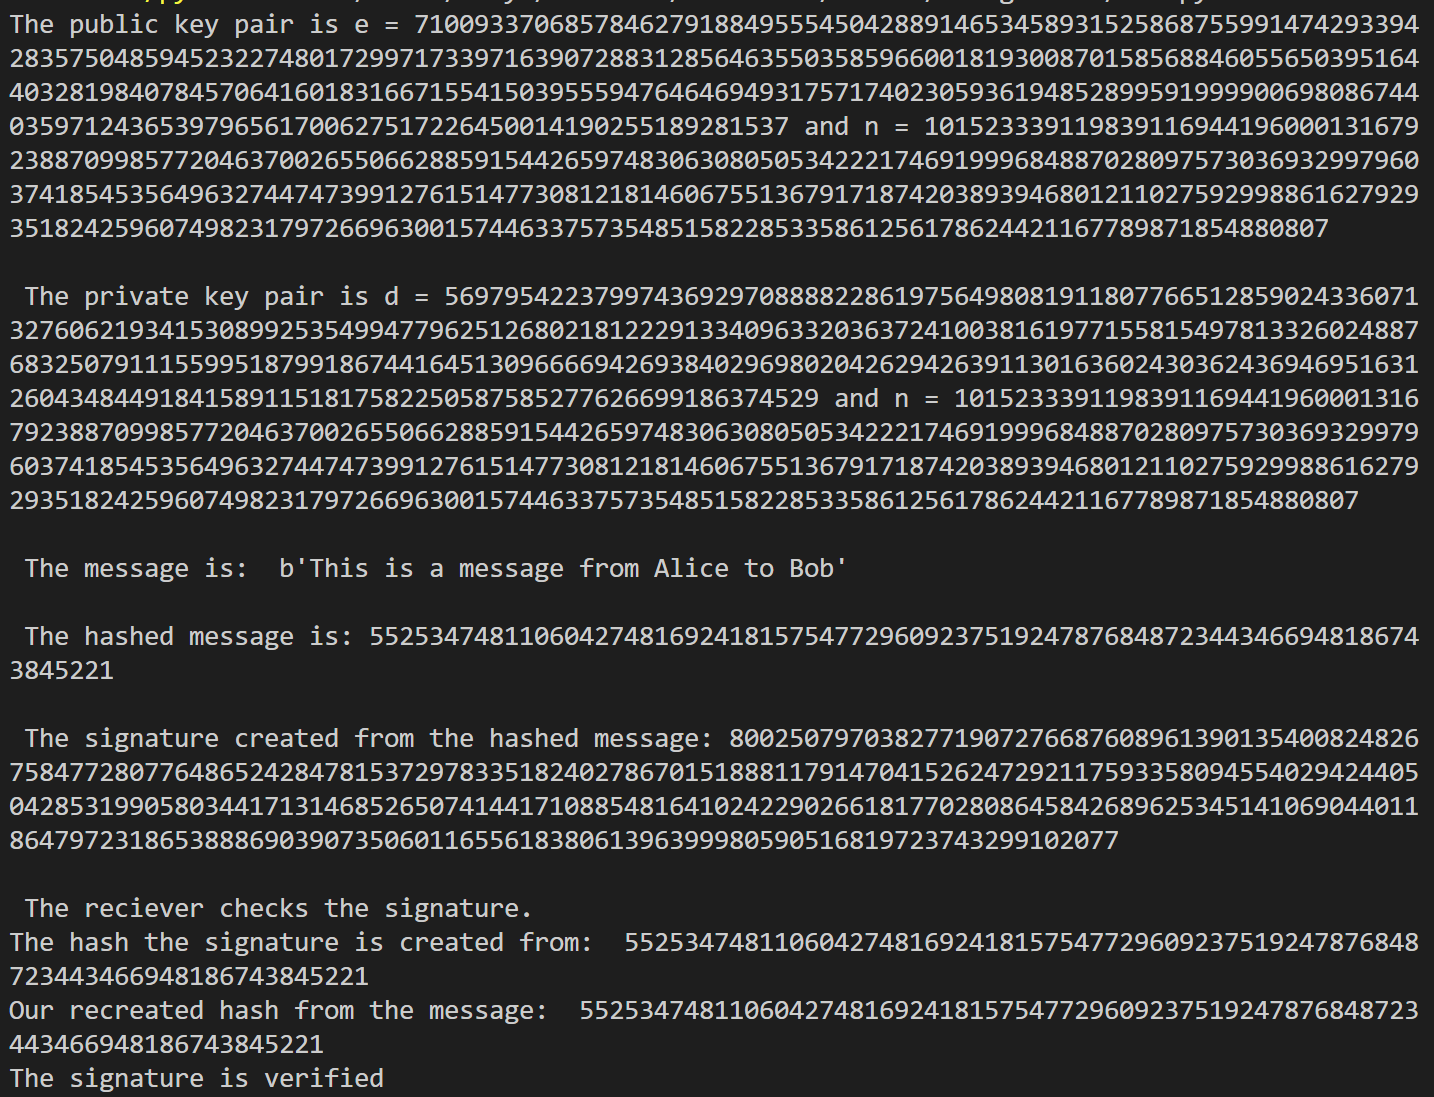
\includegraphics[width=\linewidth]{code_snippets/print.PNG}\centering
  \caption{The print statements from the RSA.py main}
  \label{fig:print}
\end{figure}

Using this on the two applications will look as shown in Figure \ref{fig:msg}, when the signature is verified. If the signature does not match the message, the note under the message will tell you that.

\begin{figure}[H]
  \hspace*{-50px}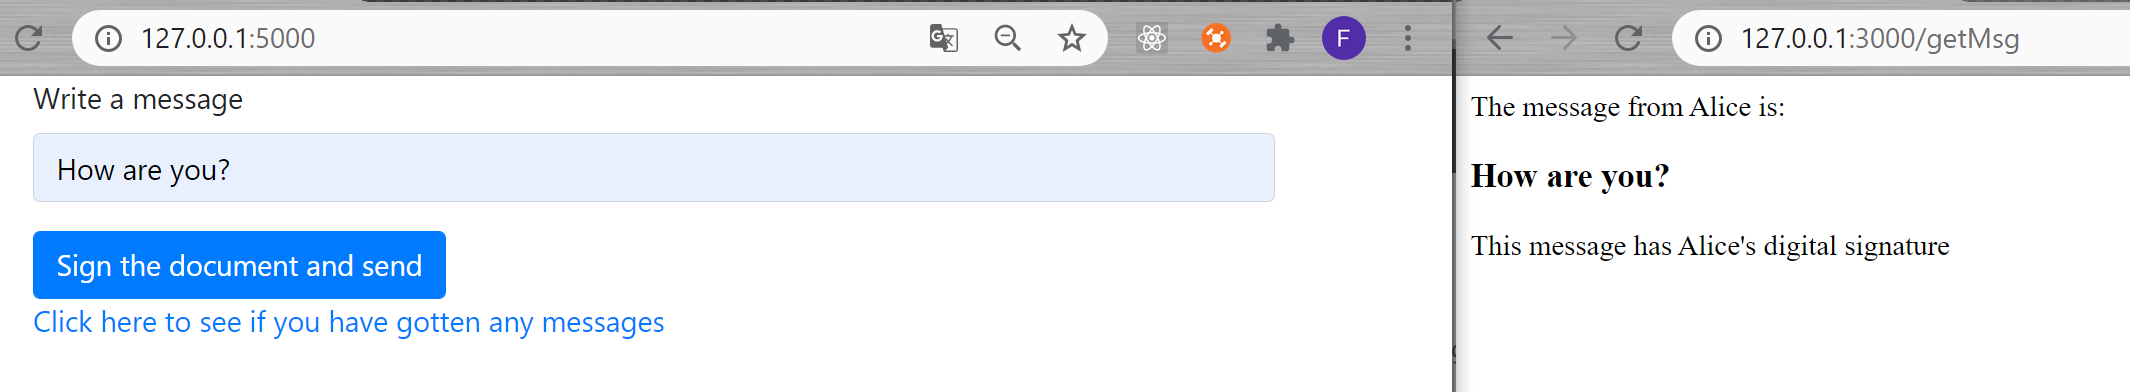
\includegraphics[width=500px]{code_snippets/msg.PNG}\centering
  \caption{Alice sends a message and sign it. Bob receives it and verifies the signature}
  \label{fig:msg}
\end{figure}

It seems like RSA usually uses keys of 2048 bits. Creating and working with that big numbers goes slow in python and to beware of computational problems I have used the package \textit{timeit} to find out the different execution times depending on the bit length. You can see the result in the table here.

\begin{center}
\begin{tabular}{ |c|c|c| } 
 \hline
 Bit length & Execution time\\
 128 & 0.060 \\ 
 256 & 0.186 \\ 
 512 & 0.738 \\ 
 1024 & 4.894 \\ 
 2048 & 35.01 \\
 \hline
\end{tabular}
\end{center}

As you can see in the table, the execution time increases exponentially as we increase the bit length. But the important thing here is that if the product of p and q is bigger than the hashed message, which is 256-bits, or else this will not work. So when I tested with 128bit primes to create the key, the digital signature did not work. A way to solve that is to split up the keys or split up the message and create a longer hash, but I chose to not do that because the execution time of keys created from larger primes is not that small.

\section*{Discussion}
The keys are created and fulfill the requirements to work in RSA. The RSA digital signature does work as expected and I think the result is good. With the keys created I could also have used them for encrypting and decrypting messages. I have chosen to use a default of 512-bit primes as \textbf{p} and \textbf{q}, because that's small enough to test the application without having to wait for the program to run but large enough to provide some security and works without splitting the keys. 
I could have, and was thinking about splitting up the message, to get a lower execution time, but did not see that as a must in this case, since the messages were not that big anyway. I tried sending a string with 5000 characters, and it was slower, but nothing crucial. With more time I think it had been fun to try to implement SHA256 from the bottom, but that is for later when I have some extra time. 

\section*{Part 2}
\textit{1. What are the different types of SSL's and how different they are in aspect of security? Why ?}\\
SSL (Security Sockets Layer) does encrypt data that is transferred between users and a website. Because it ensures that malicious third parties can't intercept your personal information it is especially important if the website features facilities as logins, forms that capture personal data or Credit card transactions. There are different types of SSL certificate but all of them have the same level of encryption. The differences is the level of validation. Validation level refers to the extent of checks that a Certificate Authority (CA) does to verify the identify of a person or organization that owns a website. I will get back to the CA in the next question. There are three main types of SSL validation:
\\ 
\textbf{Domain Validated certificates (DV SSL)}
\\
DV SSL is the lowest level of validation of these three. When you get the certificate, CAs does not look into information about the person or company that is running the website. They just check that they have control over the domain that is want's to be SSL certified. As a user, there is therefore limited information about the website ownership. For the person or organization issuing the certificate this is a quick process which is generally online and automated. It is also the cheapest option.
\\
\textbf{Organization validated certificates (OV SSL)}
\\
OV SSL requires some background checks. The CAs has to verify the individual or business that own the domain and do a minor evaluation. This is more trustworthy that DV SSL because the users can click on the padlock display and get some information about the owners of the domain, such as name, address and country. The users do therefore know who they are giving their information to. It takes often several days to issue an OV SSL cert, since some checks have to be done.
\\
\textbf{Extended Validated certificates (EV SSL)}
\\
EV SSL is the highest level of SSL certification you can get. CAs does extensive background cheks on the owners, validating its ownership, legal existence, physical location, and more. This is very expensive and can often take several weeks to issue. But with a EV cert the users will have no doubt about the site's trustworthiness and that it is a legitimate business.
\\
Depending on how many domains you need there is different types of SSL certificates. Each SSL cert combines the level of validation with the number of domains. Based on how many domains you need there are four different types of SSL.
\\
\textbf{Single-domain SSL certificate}
\\
With this certificate a single domain and all the pages on that domain are protected. You can choose between all three different validation levels for this certificate.
\\
\textbf{Wildcard SSL certificate}
\\
With this certificate you can protect a single domain and unlimited subdomains for that domain. This certificate can be issued with DV and OS level of validation, but not EV.
\\
\textbf{Multi-Domain SSL certificate}
\\
With this certificate you can protect up to 100 different domains. Wildcard domains can also be protected with a multi-domain SSL certificate. All three validation levels are available for this certificate.
\\
\textbf{Unified Communications SSL certificate}
\\
This certificate are similar to multi-domain certificates and can secure up to 100 domains and subdomains on one certificate. But unified communication certificates are created specifically for environments that utilize Microsoft Exchange and Office Communications. They use the Subject Alternative Name (SAN) extension instead of different IP address to secure these domains.
\\\\
By combining a validation level appropriate to the purposes, with the number of domains you need you can get an optimal SSL certificate. For answering this question I have used an article from namecheap.com and it's references, read it here \cite{ssl}.
\\\\
\textit{2. Research about the the Certificate Authority Security concerns and explain.}\\
A certificate authory (CA) is a company or organization that acts to validate the identities of entities such as websites, email addresses, companies, or individual persons and bind them to cryptographic keys through the issuance of electronic documents known as digital certificates. A digital certificate verifies the ownership of a public key by the named subject of the certificate. A CA acts as a thrusted third part, which both the owner of the certificate and the party relying upon the certificate must trust. Sertifikatene varer for lenge. Let's 
\\
Single point of failure - hvem som helst kan lage en CA
\\
Problem with CA behaviour badly
\\
Lack of transparency - CA browser forum
\\
Breach - en private key blir lekket
\\
\textit{3. How does browsers identify secure CA's From another CA's and how is it measured ?}\\
For the browser to identify and differ between CA's it needs access to the entire certificate chain up to and including the root CA for all of certificates it will verify. The root certificate must have been issued in a secure way. An other method used is to use the certificate trust list (CTL). That's a list of all trusted certificates. The list has to bee signed by the root CA that the browser trust. If one of the private keys in the certificate three has been lost or revealed, all of the children of that certificate can not be used anymore. 
sjekk datoen


\section*{Conclusion}
A short paragraph that restates the objective from your introduction and relates it to your results and discussion, and
describes any future improvements that you would recommend. Works Cited A bibliography of all of the sources
you got information from in your report. 


\begin{thebibliography}{10} 
\bibitem{65537} 65,537,  \emph{Wikipedia - The number 65537},
\url{https://en.wikipedia.org/wiki/65,537}.
\bibitem{modinv} GeeksforGeeks,  \emph{Modular inverse},
\url{https://www.geeksforgeeks.org/multiplicative-inverse-under-modulo-m/}.
\bibitem{ssl} NameCheap,  \emph{Types of SSL Certificates},
\url{https://www.namecheap.com/security/ssl-certificate-types/}.
\end{thebibliography}



\end{document}